\begin{enumerate}
\def\labelenumi{\arabic{enumi}.}

\item
  toc \{:toc\}
\end{enumerate}

\textbf{Subpages:}

\begin{itemize}

\item
  \href{outline.html}{Outline}
\item
  \href{todo.html}{TODO}
\item
  \href{scraps.html}{Scraps}
\end{itemize}

\{\% include acknowledgements.html \%\}

\{\% include foreword.html \%\}

\hypertarget{introduction}{%
\section{Introduction}\label{introduction}}

The world is Big Data, and The Cloud is its landlord. Much like the
universal commodification of prior \cite{warkCapitalDeadThis2021}  assemblages of capitalism, The Cloud's informational capitalism
recasts every element of our reality as Data, and it is our
responsibility to ferret it out of its primitive unknown, mine it,
harvest it, dump it by the tanker-truckful into great Data Lakes and
wring the Actionable Insights from its neck. The world has always been
Big with Data, but The Cloud has finally given us a fruit of knowledge
to munch on that reveals its true nature. We are but Data Subjects, and
if we can harness the wily spray of our Organic Content with biosensor
wearables, filtering our every action, affection, and affilitation
through a mob of algorithmically optimized platforms, then The Cloud
might teach us enough about ourselves to be able to lead a fulfilled and
healthy life. Academics and Governments in particular are filthy with
Data, and have set their eyes on a new generation of data
infrastructures that promise to dissolve the Silos that prevent the Big
Data from teaching us the nature of the universe, how to solve poverty,
reverse climate change, and finally collapse into one great cat-pile of
peace and love for our neighbor. The Cloud is dreaming of linking the
Big Data into one great Knowledge Graph of Everything --- it tells us
this is important for the fate of humanity.

The Knowledge Graph of Everything is a mirage, though. Its vision of
extracting all the world's data is the same colonial vision of infinite
prosperity that has driven us to the brink of extinction: So The Cloud
Said, let us make Platforms in our image, and let them have dominion
over the interactions with the apps, and the insights of the analytics,
and over all the data of the earth. The pursuit of universalizing
ontologies that will finally give every quantum of Data its one True and
Correct form is the same fascistic vision that has driven eliminationist
campaigns to stamp out degeneracy: Ontologien über alles. Aside from its
properly pathological nature, the Knowledge Graph of Everything \emph{is
impossible} and \emph{won't work.} Instead, The Cloud will lead
governments and academics along by the nose just long enough to build
critical mass for an interlocking set of platforms that slice off
snapshots of the Everything to ratchet us ever futher into the captivity
of surveillance and subscription.

What is the alternative? The Cloud presents its future as inevitable,
but by seeing past its logic we might imagine properly \emph{human}
infrastructures that fill the needs for connection and understanding
that it exploits. This piece develops the notion of \textbf{vulgar
linked data} as an alternative to the Cloud Orthodoxy. Predicated on
relationality, heterogeneity, privacy, and vernacular expression, vulgar
linked data infrastructures attempt to empower \emph{people} to
\emph{socially organize} information in a truly decentralized
sociotechnological commons, rather than empowering \emph{systems} to
\emph{rent} knowledge organization for \emph{profit.}

\hypertarget{knowledge-graphs-a-backbone-in-the-surveillance-economy}{%
\section{Knowledge Graphs: A Backbone in the Surveillance
Economy}\label{knowledge-graphs-a-backbone-in-the-surveillance-economy}}

Through their cloud of corporate jargon, knowledge graphs are relatively
straightforward to define \cite{chaudhriKnowledgeGraphsIntroduction2022, hitzlerReviewSemanticWeb2021, yanRetrospectiveKnowledgeGraphs2018, bergmanCommonSenseView2019} 
(though see \cite{ehrlingerDefinitionKnowledgeGraphs2016} ):
\textbf{directed, labeled graphs} consisting of \emph{nodes}
corresponding to entities like a person, dataset, location, etc. and
\emph{edges} that describe their relationship\footnote{Equivalently, one
  could emphasize that they are graphs composed of \textbf{triplet}
  links that describe some subject, predicate, and object.}. Knowledge
graphs typically make use of some controlled \textbf{ontology} that
provide a specific set of terms and how they are to be used, and
``types'' that give a given entity an expected set of \emph{properties}
denoted by edges with a particular set of labels from the ontology. For
example, the schema.org \href{https://schema.org/Person}{Person} type
would be applied to a node, and then have a set of labeled edges like
\texttt{gender} or \texttt{email} that link to other nodes that contain
the values of the properties.

Why does such a seemingly ordinary data structure deserve particular
attention in an always-more-fraught landscape of digital technology? The
story of knowledge graphs is the story of the enclosure of the wild and
open web into a series of surveillance-backed platforms. They provide an
underexplored lens onto the present and future of digital infrastructure
as planned by information conglomerates --- and serve as a liberatory
kernel that hints at how we might chart a different course.

\hypertarget{semantic-web-priesthoods}{%
\subsubsection{Semantic Web:
Priesthoods}\label{semantic-web-priesthoods}}

The term ``Knowledge Graph'' evolved out of the Semantic Web project
\cite{hitzlerReviewSemanticWeb2021} . It is difficult to
reconstruct how radical the notion of a collection of documents
organized by arbitrary links between them was at dawn of the internet.
At the time, the infrastructures of linking documents looked more like
ISBNs, carefully regulated by expert, centralized
authorities\footnote{For another example re: the political nature of the
  DOI system in the face of the arbitrary linking of the internet, see
  section 3.1.2
  ``\href{https://jon-e.net/infrastructure/\#seemingly-prosocial-protocols-can-be-used-by-industries-to-preem}{Integration,
  not Invention}'' in \cite{saundersDecentralizedInfrastructureNeuro2022} }. Being able to
\emph{just make anything that could be linked to} and \emph{link to
anything you wanted} was \emph{terrifying} and \emph{new} (eg. \cite{berners-leeLinksLaw1997, berners-leeLinksLawMyths1997} ).

The initial design of the web imagined it as a self-organizing process,
where people would maintain their own websites and organize a collection
of links to other websites. It became clear relatively quickly that the
anarchy of a socially self-organizing internet wasn't going to work as
planned, where without a formal system of organization ``people were
frightened of getting lost in it. You could follow links forever.'' \cite{berners-leeWhatSemanticWeb1998} 

In its earliest formulations, the Semantic Web was an attempt to
supplement the same arbitrary power to express human-readable
information with computer-readable information. It imagined a linked and
overlapping set of schemas ranging from locally expressive vocabularies
used among small groups of friends through globally shared, logically
consistent ontologies. The semantic web was intended to evolve fluidly,
like language, with cultures of meaning meshing and separating at
multiple scales \cite{berners-leeScalefreeNatureWeb1998, berners-leeSemanticWeb2001, berners-leeCulturesBoundaries2007} :

\begin{quote}
Locally defined languages are easy to create, needing local consensus
about meaning: only a limited number of people have to share a mental
pattern of relationships which define the meaning. However, global
languages are so much more effective at communication, reaching the
parts that local languages cannot. {[}\ldots{]}

So the idea is that in any one message, some of the terms will be from a
global ontology, some from subdomains. The amount of data which can be
reused by another agent will depend on how many communities they have in
common, how many ontologies they share.

In other words, one global ontology is not a solution to the problem,
and a local subdomain is not a solution either. But if each agent has
uses a mix of a few ontologies of different scale, that is forms a
global solution to the problem. \cite{berners-leeScalefreeNatureWeb1998} 
\end{quote}

\begin{quote}
The Semantic Web, in naming every concept simply by a URI, lets anyone
express new concepts that they invent with minimal effort. Its unifying
logical language will enable these concepts to be progressively linked
into a universal Web. \cite{berners-leeSemanticWeb2001} 
\end{quote}

This freeform goal expression for expression's sake was always in
tension with another part of the vision - serving as a backbone for AI
``agents'' that could compute emergent function from the semantic web.
Succinctly: ``Human language thrives when using the same term to mean
somewhat different things, but automation does not.'' \cite{berners-leeSemanticWeb2001}  This tension persists through the
broader history of the web.

\hypertarget{linked-data-platforms}{%
\subsubsection{Linked Data: Platforms}\label{linked-data-platforms}}

Much of the work of the semantic web project in the early 2000s focused
on the ``global'' side of this tension at the expense of the ``local'' -
creating ontologies and related technologies intended to serve as a
foundation for expressing basic things in a common vocabulary \cite{hitzlerReviewSemanticWeb2021} . This work had many successes, but
began a schism between the priesthood of people concerned with making
systems that were \emph{correct} and those that were more concerned with
making things that \emph{worked} - or supported ``local'' expression (eg
\cite{palmerDitchingSemanticWeb2008} ). Aaron Swartz captured
this frustration in his unfinished book:

\begin{quote}
Instead of the ``let's just build something that works'' attitude that
made the Web (and the Internet) such a roaring success, they brought the
formalizing mindset of mathematicians and the institutional structures
of academics and defense contractors. They formed committees to form
working groups to write drafts of ontologies that carefully listed (in
100-page Word documents) all possible things in the universe and the
various properties they could have, and they spent hours in Talmudic
debates over whether a washing machine was a kitchen appliance or a
household cleaning device. \cite{swartzAaronSwartzProgrammable2013} 
\end{quote}

Lindsay Poirier describes this difference in ``thought styles'' as a
rift between the ``neats'' focused on universalizing \emph{a priori}
ontologies and the ``scruffies'' focused on everyday use and letting the
structure appear afterwards \cite{poirierTurnScruffyEthnographic2017} . The latter characterizes the ``second age'' of the Semantic Web
after 2006 - the reorganization around \textbf{Linked Data} \cite{berners-leeLinkedData2006, hitzlerReviewSemanticWeb2021} . The era of
Linked Data de-emphasized the idealistic and ideological goals of the
early Semantic Web, driven more by an empirical approach of trying to
realize these systems on the wilds of the web, creating some of the
first public ``Linked Open Data'' systems like DBPedia and Freebase.

This turn coincides with the emerging platformatization and enclosure of
the web as ``Web 2.0.'' Throughout the early 2000s, the work of the
Semantic Web project was largely invisible to the ordinary web user, and
its vision of a self-organizing web was easily outcompeted by the
now-ubiquitous use of search engines to index the web. Where in the
early 2000s web architects were imagining the future of web continuing
to take place on free and open \emph{protocols,} the Linked Data/Web 2.0
era corraled us into a pattern of \emph{platforms} which quickly
ratcheted their way to dominance in a positive feedback loop of user
experience design, network effects and profit. On platforms, rather than
a system that ``belongs'' to everyone, you are granted access to some
specific set of operations through an interface so that you can be part
of a social process of producing and curating information for the
platform holder.

\hypertarget{knowledge-graphs-panoptica}{%
\subsubsection{Knowledge Graphs:
Panoptica}\label{knowledge-graphs-panoptica}}

In 2010 Google acquired Metaweb and its publicly-edited Semantic Web
database Freebase, and in 2012 repackaged it and the ideas of Linked
Data as what it called a \textbf{Knowledge Graph} --- the third era of
the Semantic Web \cite{singhalIntroducingKnowledgeGraph2012, iainFreebaseDeadLong2016} . Freebase only made up part of it, and the
full extent of Google's Knowledge Graph are unknown, but its most
visible impact are the factboxes that present structured information
about the subjects of searches - like biographical information in a
search for a person - or the different widgets for contextual
interaction - like being able to make a restaurant reservation from the
serach page \cite{noyIndustryscaleKnowledgeGraphs2019} .
Knowledge Graphs still share the same underlying structure --- triplet
graphs with ontologies --- even if they occupy a broader space of
implementations and technologies. What differs is the context and
intended use: the ``worldview'' of the knowledge graph.

Beyond the obvious product-level features it supports, Google's
acquisition of Freebase and the structure of its Knowledge Graph
represent at least two deeper shifts in the trajectory of the Semantic
Web and the broader internet: the privatization of technologies with
initially liberatory aspirations, and an early template of the
sprawling, surveillance-driven information conglomerate we know and love
today.

Like the radical nature of linking on the web, it's difficult to
remember that the web as surveillance apparatus thinly veiled as the
five or so remaining websites was not inevitable. The pre-dotcom bust
internet of the 90's and early 2000's was far from the commercialized
wasteland we know today. Ed Horowitz, CEO of Viacom explained in 1996:
``The Internet has yet to fulfill its promise of commercial success.
Why? Because there is no business model'' \cite{tarnoffInternetPeopleFight2022} . Google's AdWords being a defining
moment in the development of surveillance capitalism is a story already
told \cite{zuboffAgeSurveillanceCapitalism2019} : taking
advantage of the need for search generated by the disorganization of the
web, AdWords turned personal search data into a profit vector by selling
targeted space in the results.

The significance of the relationship between search, the semantic web,
and what became knowledge graphs is less widely appreciated. The
semantic web was initially an alternative to monolithic search engine
platforms - or, more generally, to platforms in general \cite{berners-leeSociallyAwareCloud2009} . It imagined the use of triplet
links and shared ontologies at a protocol level as a way of organizing
the information on the web into a richly explorable space: rather than
needing to rely on a search bar, one could traverse a structured graph
of information \cite{berners-leeLinkedData2006, berners-leeGoalsHumanDataInterface2010}  to find what one needed
without mediation by a third party.

Instead, the form of of the semantic web that emerged as ``Knowledge
Graphs'' flipped the vision of a free and evolving internet on its head.
The mutation from ``Linked Open Data'' \cite{berners-leeLinkedData2006}  to ``Knowledge Graphs'' is a shift in
meaning from a public and densely linked web of information from many
sources to a proprietary information store used to power derivative
platforms and services. The shift isn't quite so simple as a ``closure''
of a formerly open resource --- we'll return to the complex role of
openness in a moment. It is closer to an \emph{en}closure, a
\emph{domestication} of the dream of the Semantic Web. A dream of a
mutating, pluralistic space of communication, where we were able to own
and change and create the information that structures our digital lives
was reduced to a ring of platforms that give us precisely as much agency
as is needed to keep us content in our captivity. Links that had all the
expressive power of utterances, questions, hints, slander, and lies were
reduced to mere facts. We were recast from our role as \emph{people}
creating a digital world to \emph{consumers} of subscriptions and
services. The artifacts that we create for and with and between each
other as the substance of our lives online were yoked to the acquisitive
gaze of the knowledge graph as \emph{content} to be mined. We vulgar
commoners, we data subjects, are not allowed to touch the graph --- even
if it is built from our disembodied bits.

The same technologies, with minor variation, that were intended to keep
the internet free became emblematic of and coproductive with the
surveillance/platform model that has enclosed it. Beyond Google,
knowledge graphs are an elemental part of the contempory information
economy. Banks, militaries, governments, life science corporations,
journalists, everyone is using knowledge graphs \cite{neo4jNeo4jCustomers, enterpriseknowledgegraphfoundationKnowledgeGraphIndustry2022} . Their
ubiquity is not an accident, one of many possible data systems that
could have fit the bill, but reflects and reinforces basic patterns of
the information economy and the corporations within it.

What makes knowledge graphs so special? It turns out that semantic web
technologies, designed to accomodate the infinitely heterogeneous,
multiscale nature of free and unmediated social structuring of
information are also quite useful for the indefinitely expanding dragnet
of data collection that defines the operation of contemporary
capitalism:

\begin{quote}
``If one takes a look at the top Fortune 500 companies, it is surprising
how many of them are really in the information business. I don't just
mean the technology and telecommunication companies like Apple or Google
or Verizon or Cisco or the drug companies like Pfizer. One could also
think of the big banks as a subset of the vectoralist class rather than
as ``finance capital.'' They too are in the information asymmetry
business. And as we learned in the 2008 crash, even the car companies
are in the information business---they made more money from car loans
than cars. The military---industrial sector is also in the information
business. The companies that appear to sell actual things, like Nike,
are really in the brand business. Walmart and Amazon compete with
different models of the information logistics business. Even the oil
companies are in part at least in the
information-about-the-geology-of-possible-oil-deposits business. Perhaps
the vectoralist class is no longer emerging. Maybe it is the new
dominant class.'' \emph{- McKenzie Wark, Capital Is Dead: Is This
Something Worse?} \cite{warkCapitalDeadThis2021} 
\end{quote}

Data companies --- most major companies --- need to store and maintain
massive collections of heterogeneous data across their byzantine
hierarchies of executives, managers, and workers. This gigantic haunted
ball of data is not just a tool, but the \emph{substance} of the
company. A data company persists by exploiting the combinatorics of its
data hoard, spinning off new platforms that in turn maintain and expand
access to data by creating captive data subjects\footnote{Facebook
  describes the notion of its platform as being just a means of
  interacting with its underlying data graph in corporate web design
  speak: ``A useful tool for Facebook has been to think of the graph as
  the model and a Facebook page as the view---a projection of an entity
  or collection of entities that reside in the graph.'' \cite{noyIndustryscaleKnowledgeGraphs2019} }. As it expands, a
conglomerate will acquire many new sources and modalities of data and
need to integrate them with its existing data.

Knowledge graphs are particularly well suited for this ``data
integration'' problem. A full technical description is out of scope
here, but briefly: traditional relational database systems can be very
difficult to modify and refactor, and that difficulty increases the
larger and more complex a database is\footnote{For a practical example,
  see a recent
  \href{https://www.etsy.com/codeascraft/scaling-etsy-payments-with-vitess-part-1--the-data-model}{trio}
  of
  \href{https://www.etsy.com/codeascraft/scaling-etsy-payments-with-vitess-part-2--the-seamless-migration}{blog}
  \href{https://www.etsy.com/codeascraft/scaling-etsy-payments-with-vitess-part-3--reducing-cutover-risk}{posts}
  from Etsy engineers that describe the process of scaling their
  database system.}. One has to be design the structure of the
anticipated data in advance, and the abstract schematic structure of the
data is embedded in how it is stored and accessed. It is particularly
difficult to do unanticipated ``long range'' analyses where very
different kinds of data are analyzed together.

In contrast, merging graphs is more straightforward\footnote{\begin{quote}
  That is because knowledge graphs aim to solve the data incongruence
  problem, which is one of the biggest operational headaches for
  corporates, says Atkin. ``Corporates suffer from technology
  fragmentation and as a result have a lot of data that doesn't align
  across the organization. Doing the hard work to fix this data
  incongruence reality is a pre-requisite for realizing business
  value,'' he says. \cite{schenkerNewReportDetails2021} 
  \end{quote}} \cite{chaudhriKnowledgeGraphsIntroduction2022, enterpriseknowledgegraphfoundationKnowledgeGraphIndustry2022, schenkerNewReportDetails2021, sequedaDesigningBuildingEnterprise2021, azziniAdvancesDataManagement2021, segaranTwophaseConstructionData2020, ceravoloBigDataSemantics2018, natarajanGraphKnowledgeGraph}  - the
data is just triplets, so in an idealized case\footnote{I am aware graph
  databases are not magic and this is an extraordinarily simplified
  example. The principle is the point, not all the subtle ways the
  implementations of graph databases are hard.} it is possible to just
concatenate them and remove duplicates (eg. for a short example, see
\cite{allemangMergingDataGraphs2022, allemangMergingTablesHard2022} ). The graph can be operated on locally, with more global
coordination provided by ontologies and schemas, which themselves have a
graph structure \cite{villazon-terrazasKnowledgeGraphFoundations2017} . Discrepancies between graphlike schema can be resolved by, you
guessed it, making more graph to describe the links and transformations
between them. Long-range operations between data are part of the basic
structure of a graph - just traverse nodes and edges until you get to
where you need to go - and the semantic structure of the graph provides
additional constraints to that traversal. Again, a technical description
is out of scope here, graphs are not magic, but they are well-suited to
merging, modifying, and analyzing large quantities of heterogeneous
data.

Another way of looking at the capacity for heterogeneity in triplet
graphs is by thinking of links as statements:

\begin{quote}
One person may define a \texttt{vehicle} as having a
\texttt{number\ of\ wheels} and a \texttt{weight} and a \texttt{length},
but not foresee a \texttt{color}. This will not stop another person
making the assertion that a given car is \texttt{red}, using the color
vocabulary from elsewhere. \cite{berners-leeWhatSemanticWeb1998} 
\end{quote}

So if you are a data broker, and you just made a hostile acquisition of
another data broker who has additional surveillance information to fill
out for the people in your existing dataset, you can just stitch those
new properties on like a fifth arm on your nightmarish data
frankenstein.

What does this look like in practice? While in a bygone era Elsevier was
merely a rentier holding publicly funded research hostage for profit,
its parent company RELX is paradigmatic of the transformation of a more
traditional information rentier into a sprawling, multimodal
surveillance conglomerate (see \cite{lamdanDataCartelsCompanies2023} ). RELX proudly describes itself as a gigantic haunted graph of
data:

\begin{quote}
Technology at RELX involves creating actionable insights from big data
-- large volumes of data in different formats being ingested at high
speeds. We take this high-quality data from thousands of sources in
varying formats -- both structured and unstructured. We then extract the
data points from the content, link the data points and enrich them to
make it analysable. Finally, we apply advanced statistics and
algorithms, such as machine learning and natural language processing, to
provide professional customers with the actionable insights they need to
do their jobs.

We are continually building new products and data and technology
platforms, re-using approaches and technologies across the company to
create platforms that are reliable, scalable and secure. \textbf{Even
though we serve different segments with different content sets, the
nature of the problems solved and the way we apply technology has
commonalities across the company.} \cite{relxAnnualReport20222023} 
\end{quote}

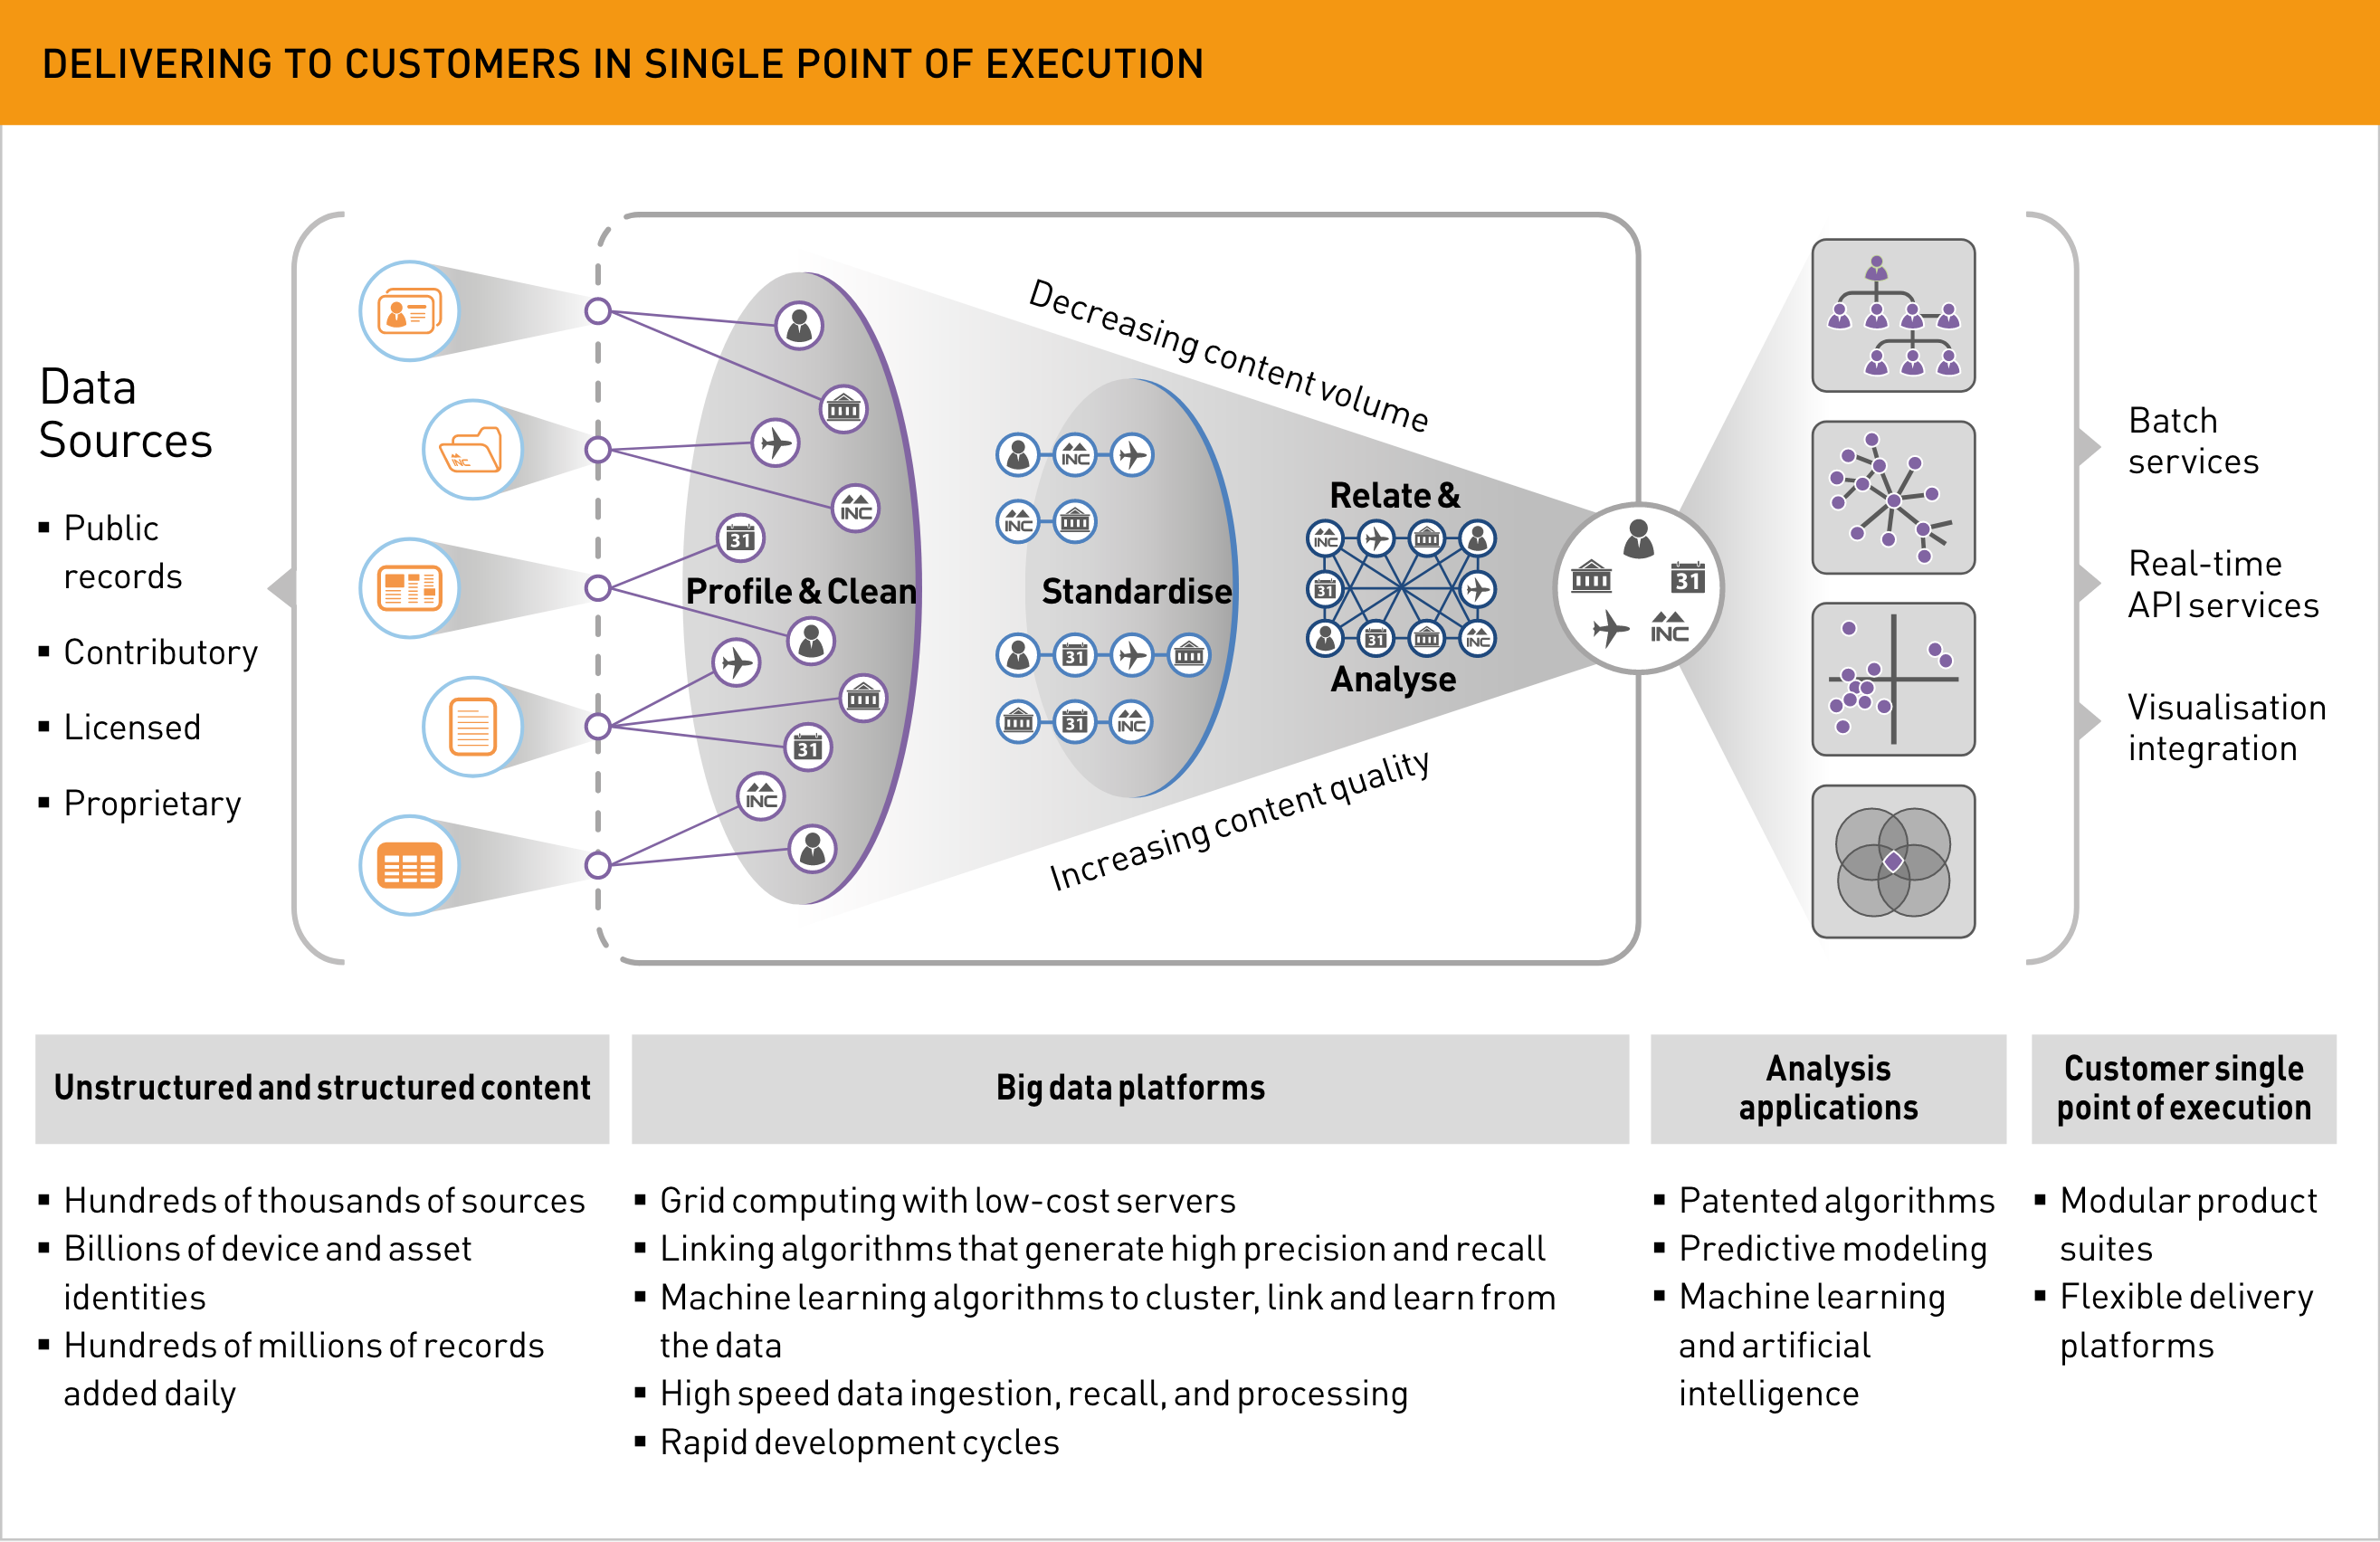
\includegraphics[width=\linewidth]{img/RELX_Pipeline_2022.png}
\emph{In its 2022 Annual Report, RELX describes its business model as
ingesting large quantities of data, linking them together, and deriving
platforms from them. \cite{relxAnnualReport20222023} }

While to any individual market segment or class of customers RELX and
its subsidiaries might look like a portfolio of separate platforms and
applications, one can only make sense of the company by thinking of each
of them as a view on an interconnected graph of data\footnote{Though
  apparently they have had historical difficulty actually getting that
  integration to work \cite{schonfeldReorganizationElsevier2022} .}. Each additional source of data, either by acquiring new
companies or by expanding their existing control of informational access
points has the potential to create some combinatorically new set of
opportunities for new platforms.

For example, RELX is able to gather surveillance data on researcher
attention data through the tracking in its ScienceDirect and Mendeley
platforms. It also collects a large amount of chemical data through its
control of scientific publishing that it rents access to on its
\href{https://www.elsevier.com/en-gb/solutions/reaxys}{Reaxys} platform,
which is supplemented by its LexisNexis PatentSight database of patents.
So far so normal.

What about the other sides of the multisided market? RELX is able to
combine these and other data sources into new product. For
pharmaceutical R\&D companies, their bespoke
\href{https://web.archive.org/web/20211207070524/https://www.elsevier.com/solutions/professional-services/drug-design-optimization}{Drug
Design Optimization} services advertise being able to use chemical,
disease, and literature-based data to generate a priority list of
potential therapeutic targets and drugs, as well as provide
``competitive intelligence'' about which targets are currently being
studied, presumably identified from their ownership of the scientific
literature coupled with surveillance data. Since clinicians don't trust
pharmaceutical advertisements \cite{elsevierMakingMedicalInformation2021} , Elsevier uses its position as
a perceived neutral third party to repackage advertisements as
informational systems \cite{elsevierRethinkClincalContent2020} ,
``journal-branded webinars,'' as well as a number of other avenues via
its
``\href{https://web.archive.org/web/20211111211058/https://www.elsevier.com/advertising-reprints-supplements/advertising}{360
degree advertising solutions}'' catalogue. So, by combining several data
sources and platforms, Elsevier is able to offer pharmaceutical
companies recommendations for candidate drugs above and beyond what
would be possible with chemical information alone and then advertise
their drugs directly to doctors.

Derivative platforms beget derivative platforms. Its integration into
clinical systems by way of reference material is growing to include
\href{https://web.archive.org/web/20230307020432/https://www.elsevier.com/en-gb/clinical-solutions/clinical-practice}{electronic
health record} (EHR) systems, and they are ``developing clinical
decision support applications {[}\ldots{]} leveraging {[}their{]}
proprietary health graph'' \cite{relxAnnualReport20222023} .
Similarly, their integration into Apple's watchOS to track medications
indicates their interest in directly tracking personal medical data.

That's all within biomedical sciences, but RELX's risk division also
provides ``comprehensive data, analytics, and decision tools for
{[}\ldots{]} life insurance carriers'' \cite{relxAnnualReport20222023} , so while we will never have the kind of
external visibility into its infrastructure to say for certain, it's not
difficult to imagine combining its diverse biomedical knowledge graph
with personal medical information in order to sell risk-assessment
services to health and life insurance companies. LexisNexis has personal
data enough to serve as an ``integral part'' of the United States
Immigrations and Customs Enforcement's (ICE) arrest and deportation
program \cite{biddleLexisNexisProvideGiant2021, biddleICESearchedLexisNexis2022} , including dragnet
\href{https://web.archive.org/web/20230308034123/https://risk.lexisnexis.com/products/accurint-trax}{location
data} \cite{lexisnexisrisksolutionsAccurintTraX} ,
\href{https://risk.lexisnexis.com/products/telematics-ondemand}{driving
behavior data} from internet-connected cars \cite{lexisnexisrisksolutionsTelematicsOnDemand} , and
\href{https://risk.lexisnexis.com/products/threatmetrix}{payment and
credit data} as just a small sample from its large
\href{https://web.archive.org/web/20230308034302/https://www.lexisnexis.com/pdf/AccurintForLegalProfessionals/24.pdf}{catalogue}
\cite{lexisnexisrisksolutionsAccurintLegalProfessionals2022}  of
data \href{https://risk.lexisnexis.com/our-technology/lexid}{aggregated
and linked} into comprehensive profiles \cite{lexisnexisrisksolutionsLexID} . The contemporary knowledge
graph-powered surveillance conglomerate gains its versatility precisely
from its ability to span many unrelated domains and deploy new platforms
as opportunities present themselves. As new data sources are acquired,
the combinatorics of possible surveillance products correspondingly
explode.

This pattern is true across the information industry \cite{sequedaDesigningBuildingEnterprise2021} . A handful of
representatives from Microsoft, Google, Facebook, eBay, and IBM describe
some elements of each of their knowledge graphs in a 2019 paper \cite{noyIndustryscaleKnowledgeGraphs2019} . Each has different
scopes, applications, and interaction with the other data and processing
infrastructure at the company, but all emphasize the ability for their
knowledge graphs to accomodate change, heterogeneity, conflicting data,
inference, and facilitate work by distributed teams due to their
self-documenting and modular nature. Neo4j, developers of an eponymous
graph database library, describes in one
\href{https://neo4j.com/case-studies/us-army/}{case study} among its
\href{https://neo4j.com/customers/}{hundreds of customers} how the U.S.
Army uses its ``connected data'' to track its equipment and estimate the
cost of some new exploratory imperialism \cite{neo4jNeo4jArmyCase2021} . An analysis of Palantir's hundreds of
patents for knowledge graph technology (eg. \cite{cohenSystemMethodSharing2015, mathuraAutomatedDatabaseAnalysis2017, yousafSystemsMethodsUser2018, knudsonSystemsMethodsAnnotating2021} )
describes its ambitions for its knowledge graph:

\begin{quote}
There is evidence {[}\ldots{]} that Palantir has infrastructural
aspirations to become a general classification system for data
integration {[}\ldots{]} that can be tailored into a universal knowledge
graph. {[}\ldots{]} Palantir similarly imagines a world where its
platform might serve as a ``shadow'' universal knowledge graph for
governments, industries, and organizations. \cite{iliadisSeerSeenSurveying2022} 
\end{quote}

Knowledge graphs \emph{as a technology} - like all technologies - are
not intrinsically unethical. It is the structure of the capital-K
capital-G Knowledge Graph \emph{as a concept} with its \emph{context}
that is pathological. They represent the historical trajectory of
semantic web ideas and technologies from something that we are intended
to use and create directly into privately held data that we can only
interact with through platforms. They are coproductive with the
corporate and technical structure of surveillance capitalism,
facilitating conglomerates that gobble up as many platforms and data
sources as possible to stitch them into an expanding, heterogeneous
graph of data. We will return to the underlying ideology of the
knowledge graph and an alternative in the final section.

In particular, it is their ``graph plus compute'' structure - where some
underlying graph of data is coupled with a set of algorithms and
interfaces to view it - that is necessary to understand some of the more
counterintuitive motivations of surveillance conglomerates. This
structure complicates questions of ``openness'' versus
``proprietariness,'' one of the deepest loci of criticism of the
platformatized web, and provides a different lens on ostensibly ``open''
or ``public'' knowledge graph-based infrastructure projects.

\hypertarget{public-graphs-private-profits}{%
\section{Public Graphs, Private
Profits}\label{public-graphs-private-profits}}

\hypertarget{unqualified-openness-considered-harmful}{%
\subsubsection{Unqualified Openness Considered
Harmful}\label{unqualified-openness-considered-harmful}}

A reader that I am constructing as a straw man for the sake of argument
might ask: if the problem is information conglomerates stockpiling a
massive quantity of proprietary data and renting use of it, isn't ``open
data'' the answer? And to that reader I would gently shake my head and
say a qualified ``no.''

``Openness,'' including open source, open standards, and open data, is a
subtle tool that can be used both to dissolve and reinforce economic and
political power \cite{bowkerSortingThingsOut1999} .

Free and open source software, with its noble (and decidedly
non-monolithic \cite{liuFreedomIsnFree2018} ) goal of creating an
ecosystem of free\footnote{``free as in whatever will prevent you from
  @'ing me about getting some definition of free wrong.''} software, is
a means by which large information companies can harvest the commons and
outsource labor costs \cite{warkHackerManifesto2004, goldsmithOriginalSinFree2019, hallidayOpenSourceNot2018, hunterReclaimingComputingCommons2016, hornPostOpenSource2020} . There
are countless examples of FOSS developers maintaing software widely used
by companies making billions of dollars for little or no compensation -
eg.
\href{https://github.com/zloirock/core-js/blob/master/docs/2023-02-14-so-whats-next.md}{core-js}
\cite{pushkarevWhatNext2023} ,
\href{https://veridicalsystems.com/blog/of-money-responsibility-and-pride/index.html}{OpenSSL}
\cite{marquessSpeedsFeedsMoney2014} , leftpad \cite{gallagherRagequitCoderUnpublished2016} ,
\href{https://github.com/chrisdutz/blog/blob/main/plc4x/free-trial-expired.adoc}{PLC4X}
\cite{dutzYourFreeTrial2022}  and so on. When an information
company releases or supports an open source project it is rarely an act
of altruism. The effect is to prevent another company from profiting
from a proprietary version of that technology, signal virtue, drive
recruitment, and create a centralized point to concentrate donated
labor. Microsoft, a famously
\href{https://en.wikipedia.org/wiki/Embrace,_extend,_and_extinguish}{good
actor} in software, took this several steps further with GitHub, VSCode,
and later Copilot, capturing a large chunk of the software development
\emph{process} in order to trick programmers to be the
``\href{https://twitter.com/json_dirs/status/1410897161277956097}{humans
in the loop}'' refining the neural network to write code and dilute
their labor power \cite{butterickGitHubCopilotInvestigation2022, butterickGitHubCopilotLitigation2022, olearyVSCodeWhat2022, VSCodiumOpenSource} .

``\href{https://en.wikipedia.org/wiki/Peer_production}{Peer
production}'' models, a more generic term for public collaboration that
includes FOSS, has similar discontents. The similar term
``crowdsource\footnote{For critical work on crowdsourcing in the context
  of ``open science,'' see \cite{mirowskiFutureOpenScience2018} ,
  and in the semantic web see \cite{allhutterWorkingOntologistsHighQuality2019} .}'' quite literally
describes a patronizing means of harvesting free labor via some
typically gamified platform. Wikipedia is perhaps the most well-known
example of peer production\footnote{I have written about the peculiar
  structure of Wikipedia among wikis previously, section 3.4.1 -
  ``\href{https://jon-e.net/infrastructure/\#the-wiki-way}{The Wiki
  Way}'' \cite{saundersDecentralizedInfrastructureNeuro2022} },
and it too struggles with its position as a resource to be harvested by
information conglomerates. In 2015, the increasing prevalence of
Google's information boxes caused a substantial decline in wikipedia
pageviews \cite{UserTalkJimbo2015, hinkisGoogleSteals5502015}  as
its information was harvested into Google's knowledge graph, and a
``will she, won't she'' search engine arguably intended to avoid
dependence on Google was at the heart of its 2014-2016 leadership crisis
\cite{whiteWikimediaTimelineEvents2016, buetlerSearchDestroyKnowledge2016} . After shuttering Freebase,
Google has donated a substantial amount of money to kickstart its
successor \cite{pellissiertanonFreebaseWikidataGreat2016} 
Wikidata, presumably as a means of crowdsourcing the curation of its
knowledge graph \cite{wikimediameta-wikiGoogleMeta, GoogleStakeWikidata2019, vrandecicWikidataFreeCollaborative2014} .

``Open'' standards are yet another fraught domain of openness. For an
example within academia, the seemingly-open Digital Object Identifier
(DOI) system was concocted as a means for
\href{https://jon-e.net/infrastructure/\#seemingly-prosocial-protocols-can-be-used-by-industries-to-preem}{publishers
to retain control of indexing research}, avoiding the impact of the
proposed free repository PubMedCentral and the high overhead of linking
documents between publishers\footnote{``The potential benefit of the
  service that would become CrossRef was immediately apparent.
  Organizations such as AIP and IOP (Institute of Physics) had begun to
  link to each other's publications, and the impossibility of
  replicating such one-off arrangements across the industry was obvious.
  As Tim Ingoldsby later put it, \textbf{`All those linking agreements
  were going to kill us.'}'' \cite{crossrefFormationCrossRefShort2009} } (see sec.~3.1.1 in \cite{saundersDecentralizedInfrastructureNeuro2022} ). The nonprofit
standards body \href{https://www.niso.org}{NISO}'s standards for
indicating journal article versions \cite{nisoRP82008JournalArticle2008}  and licensing \cite{nisoRP222021AccessLicense2021}  are used by publishers to enforce
their intellectual property monopolies and programmatically scour the
web to prevent free access to publicly funded information \cite{carpenterNewArticleSharing2021} .

Schema.org, a standard intended to be the generic interchange ontology
of the web, is another emblem of enclosure of the semantic web. Its
introduction at the SemTech 2011 conference was cause for a rare point
of agreement\footnote{(Intervening messages in the
  \href{https://www.w3.org/2011/06/semtech-bof-notes.html}{chat log}
  have been omitted for clarity):

  \texttt{\textless{}tantek\textgreater{}} Hey Kavi - do you see what
  you've done here? \texttt{\textless{}tantek\textgreater{}} You've
  gotten a community leader of microformats.org (myself) and chair of
  W3C RDFa WG to *agree* \texttt{\textless{}edsu\textgreater{}} tantek:
  see, that's progress :) \texttt{\textless{}manu-db\textgreater{}} Yes
  - both RDFa and Microformats communities agree - sky will be falling,
  next.} between the then-warring maintainers of RDFa and Microformats:
``folks, it's wrong for Google to dictate vocabularies, let's not lose
sight of that'' \cite{SemTech2011BOF2011} . Though ostensibly
open, its structure and emphases have been roundly criticized, eg.
having a eurocentric bias towards commercially valuable information \cite{iliadisOneSchemaRule2023} . It encourages website maintainers to
embed Schema.org annotations in their pages in exchange for a boost in
search rankings --- which Google then embeds in its infoboxes, driving
down page views. More fundamentally it cements the notion that Linked
Data is something that we are only intended to use to make our
information more available to some search engine crawler rather than
make use of for ourselves: ``In general, the design decisions place more
of the burden on consumers of the markup'' \cite{guhaSchemaOrgEvolution2015} . It encodes the notion that there should
be one ``neutral'' means of representing information for one (or a few)
global search engines to understand, rather than for local negotiation
over meaning and location. According to the transcribed Q\&A after its
2011 announcement, the Google representatives characterized the creation
of authoring tools like those created to make creative use of HTML more
accessible as a potential ``alternative path,'' but then dismissed the
notion of improved tooling as ``impossible'' \cite{hawkeNotesSessionSemTech2011} .

Clearly, on its own, mere ``openness'' is no guarantee of virtue, and
socio-technological systems must always be evaluated in their broader
context: \emph{what is open? why? who benefits?} Open source, open
standards, and peer production models do not inherently challenge the
rent-seeking behavior of information conglomerates, but can instead
facilitate it.

In particular, the maintainers of corporate knowledge graphs want to
reduce labor duplication by making use of some public knowledge graph
that they can then ``add value'' to with shades of proprietary and
personal data (emphasis mine):

\begin{quote}
In a case like IBM clients, who build their own custom knowledge graphs,
\textbf{the clients are not expected to tell the graph about basic
knowledge.} For example, a cancer researcher is not going to teach the
knowledge graph that skin is a form of tissue, or that St.~Jude is a
hospital in Memphis, Tennessee. This is known as \textbf{``general
knowledge,''} captured in a general knowledge graph. \textbf{The next
level of information is knowledge that is well known to anybody in the
domain}---for example, carcinoma is a form of cancer or NHL more often
stands for nonHodgkin lymphoma than National Hockey League in some
contexts it may still mean that---say, in the patient record of an NHL
player). \textbf{The client should need to input only the private and
confidential knowledge} or any knowledge that the system does not yet
know. \cite{noyIndustryscaleKnowledgeGraphs2019} 
\end{quote}

The creation of a collection of more domain-specific ontologies and
tooling for ingesting previously unstructured data would allow for a new
kind of globally linked knowledge graph ecosystem --- making use of a
broader range of publicly-available data, as well as facilitating new
markets for renting access to interoperable data. Five information
conglomerates conclude their joint paper on knowledge graphs
accordingly:

\begin{quote}
The natural question from our discussion in this article is whether
different knowledge graphs can someday share certain core elements, such
as descriptions of people, places, and similar entities. \cite{noyIndustryscaleKnowledgeGraphs2019} 
\end{quote}

Having such standards be under the stewardship of ostensibly neutral and
open third-parties provides cover for powerful actors exerting their
influence and helps overcome the initial energy barrier to realizing
network effects from their broad use \cite{wiegmannMultiModeStandardisationCritical2017, heiresInternationalOrganizationStandardization2008} . Peter Mika, the
director of Semantic Search at Yahoo Labs, describes this need for
third-party intervention in domain-specific standards:

\begin{quote}
A natural next step for Knowledge Graphs is to \textbf{extend beyond the
boundaries of organisations,} connecting data assets of companies along
business value chains. This process is still at an early stage, and
\textbf{there is a need for trade associations or industry-specific
standards organisations to step in,} especially when it comes to
developing shared entity identifier schemes. \cite{panExploitingLinkedData2017} 
\end{quote}

As with search, we should be particularly wary of information
infrastructures that are \emph{technically} open\footnote{Go ahead, try
  and make your own web crawler to compete with Google - all the
  information is just out there in public on the open web!} but embed
design logics that preserve the hegemony of the organizations that have
the resources to make use of them. The existing organization of
industrial knowledge graphs as chimeric ``data + compute'' models give a
hint at what we might look for in public knowledge graphs: the data is
open, but to make use of it we have to rely on some proprietary
algorithm or cloud infrastructure.

Unfortunately, that is exactly what at least two US Federal agencies
have in mind: the NIH and NSF are both in the thick of engineering
cloud-based knowledge graph infrastructures and domain-specific
ontologies with all the trappings of technology that fills the stated
needs of information conglomerates at the expense of the people it is
outwardly intended to serve. We will describe those efforts and their
already apparent risks as a way of understanding how these technologies
illustrate and reinforce the ideological and practical dominance of the
existing corporate informational ecosystem --- and to articulate an
alternative.

Add note that we are assuming that people are working with the best of
intentinos here, adn that it is hard to imagine an alternative system
when the existing one is so dominant! These are mostly good people
trying to do good things in a system that's rotten.

\hypertarget{nih-the-biomedical-translator}{%
\subsubsection{NIH: The Biomedical
Translator}\label{nih-the-biomedical-translator}}

\textbf{Note:}

This section is reproduced from, focuses, and expands on
``\href{https://jon-e.net/infrastructure/\#linked-data-or-surveillance-capitalism}{Linked
Data or Surveillance Capitalism?}'' from \cite{saundersDecentralizedInfrastructureNeuro2022} .

The NIH's Biomedical Data Translator\footnote{Or, just ``Translator''}
project was initially described in its 2016 Strategic Plan for Data
Science as a means of translating between biomedical data formats:

\begin{quote}
Through its Biomedical Data Translator program, the National Center for
Advancing Translational Sciences (NCATS) is supporting research to
develop ways to connect conventionally separated data types to one
another to make them more useful for researchers and the public. \cite{NIHStrategicPlan2018} 
\end{quote}

The original
\href{https://web.archive.org/web/20210709100523/https://ncats.nih.gov/news/releases/2016/feasibility-assessment-translator}{funding
statement from 2016} is similarly humble, and press releases
\href{https://web.archive.org/web/20210709171335/https://ncats.nih.gov/pubs/features/translator}{through
2017} also speak mostly in terms of querying the data -- though some
ambition begins to creep in. By 2019, the vision for the project had
shifted from \emph{translating} between data types into the realm of
heterogeneous linkages in some meta-level system for linking and
\emph{reasoning} over them.

In their piece ``Toward a Universal Biomedical Translator,'' then in a
feasibility assessment phase, the members of the Translator Consortium
assert that universal translation between biomedical data is
impossible\footnote{\begin{quote}
  First, we assert that a single monolithic data set that directly
  connects the complete set of clinical characteristics to the complete
  set of biomolecular features, including ``-omics'' data, will never
  exist because the number of characteristics and features is constantly
  shifting and exponentially growing. {[}\ldots{]} We also assert that
  there is no single language, software or natural, with which to
  express clinical and biomolecular observations---these observations
  are necessarily and appropriately linked to the measurement
  technologies that produce them, as well as the nuances of language.
  The lack of a universal language for expressing clinical and
  biomolecular observations presents a risk of isolation or
  marginalization of data that are relevant for answering a particular
  inquiry, but are never accessed because of a failure in translation.

  Based on these observations, our final assertion is that automating
  the ability to reason across integrated data sources and providing
  users who pose inquiries with a dossier of translated answers coupled
  with full provenance and confidence in the results is critical if we
  wish to accelerate clinical and translational insights, drive new
  discoveries, facilitate serendipity, improve clinical-trial design,
  and ultimately improve clinical care. This final assertion represents
  the driving motivation for the Translator system. \cite{consortiumUniversalBiomedicalData2019} 
  \end{quote}}\cite{consortiumUniversalBiomedicalData2019} . The
impossibility they saw was not that of conflicting political demands on
the structure of organization (as per \cite{bowkerSortingThingsOut1999} ), but of the sheer numeracy of the data
and vocabularies needed to describe them. The risk posed by a lack of a
universal ``language'' was not being able to index all possible data,
rather than inaccuracy or inequity\footnote{In an odd mixture of
  metaphors, members of the Translator consortium introduced the project
  with a piece titled ``Deconstructing the Translational Tower of
  Babel.'' \cite{austinDeconstructingTranslationalTower2019}  A
  common interpretation of the Biblical Tower of Babel is as a symbol of
  the hubris of humanity, attempting to inscribe ourselves into the
  heavens and become immune to any future God-induced flooding. God,
  concerned with the power of a humanity unified under a single
  language, punished them by scattering people into groups speaking
  mutually unintelligible languages so they would not complete the
  tower. It is unclear why an effort to create a universalizing ontology
  would then be deconstructing a tower of babel, as it was the power of
  a unified language that allowed it to be built. Perhaps in other
  interpretations the Tower is an obelisk that suppresses the
  reunification of language. But I digress.}.

Undaunted by their stated belief in the impossibility of a
universalizing ontology, the Consortium created one in their
\href{https://biolink.github.io/biolink-model/docs/}{biolink}
model\footnote{The title of the Biolink paper is ``Biolink Model: A
  universal schema for knowledge graphs in clinical, biomedical, and
  translational science'' \cite{unniBiolinkModelUniversal2022} }
\cite{bruskiewichBiolinkBiolinkmodel2021, unniBiolinkModelUniversal2022} . Biolink consists of a hierarchy of
general\footnote{General as opposed to an ontology like
  \href{https://mondo.monarchinitiative.org/}{MONDO} \cite{vasilevskyMondoUnifyingDiseases2022}  that identifies specific
  diseases.} classes: eg. a
\href{https://biolink.github.io/biolink-model/docs/BiologicalEntity.html}{BiologicalEntity}
like a
\href{https://biolink.github.io/biolink-model/docs/Gene.html}{Gene}, or
a
\href{https://biolink.github.io/biolink-model/docs/ChemicalEntity.html}{ChemicalEntity}
like a
\href{https://biolink.github.io/biolink-model/docs/Drug.html}{Drug}.
Classes can then linked by any number of properties, or
``Slots\footnote{or links, labeled edges.},'' like a therapeutic
procedure that
\href{https://biolink.github.io/biolink-model/docs/treats.html}{treats}
a disease.

Biolink was designed to be a sort of ``meta ontology,'' or a means of
mapping different domain-specific biomedical ontologies onto a common
vocabulary\footnote{To their credit, the Translator project seems to
  have made some of the long-delayed tooling for declaring a schema in a
  more accessible syntax{[}\^{}yaml{]} than RDFS/OWL and generating
  representations in multiple formats, from
  \href{https://github.com/biolink/biolink-model}{JSON-LD to pydantic
  models}. The Biolink paper also mentions a
  ``\href{https://github.com/TranslatorSRI/NodeNormalization}{Node
  Normalization Service}'' for being able to resolve Linked Data
  entities from different vocabularies that have been declared to be the
  same thing, but at the time of writing development seems to have
  \href{https://web.archive.org/web/20230316031655/https://github.com/TranslatorSRI/NodeNormalization/graphs/contributors}{slowed}}.
This design reflects the structure of the rest of the Translator
ecosystem: the interaction with domain-specific ontologies, the kinds of
data sources it uses, and the way that end users are expected to
interact with the Translator.

As a meta-ontology, biolink is targeted towards ``meta data.'' Rather
than accomodating ``raw data\footnote{In a 2018 presentation by one of
  Biolink's authors: ``What NOT to use the biolink-model for: Raw data,
  Metadata about a dataset'' with some caveat that the underlying
  metamodel might still be useful \cite{chrisIntroductionBioLinkDatamodel2018} .},'' biolink is expected to
operate at the level of ``knowledge,'' or ``generally accepted,
universal assertions derived from the accumulation of information'' \cite{fechoProgressUniversalBiomedical2022} : this procedure treats
that disease, this chemical interacts with that one, etc.

The primary way Biolink is used within the Translator is to structure a
\href{http://www.smart-api.info/registry}{registry of database APIs},
each called a ``Knowledge Source.'' Knowledge Sources use biolink to
declare that they are able to provide assertions about a particular set
of classes or slots, like
\href{http://www.smart-api.info/ui/adf20dd6ff23dfe18e8e012bde686e31}{drugs
that affect genetic expression}, which makes them part of the
Translator's distributed
\href{http://www.smart-api.info/portal/translator/metakg}{Knowledge
Graph}. The Translator project, in this universalizing impulse,
recapitulates some of the early beliefs of the Semantic Web updated with
some of the techniques of Linked Data. Since acquiring Knowledge is just
a matter of creating the right tools rather than a social process,
\href{https://reporter.nih.gov/search/DShVUhB_ZUq0X5UWFjy5WQ/projects?shared=true}{NIH
RePORTER} shows a series of grants for small councils of experts to
create domain-specific ontologies and Knowledge Sources.

This structure strongly constrains who is intended to be able to
contribute to the Translator: highly curated biomedical informatics
platforms, rather than basic researchers. This, in turn, reflects deeper
beliefs about the nature of information within the Translator ecosystem:
``knowledge'' is not a social, contextual, or dialogical phenomenon, but
a ``natural resource'' that can be
\href{https://reporter.nih.gov/project-details/10548337}{mined} from
information that is ``out there.'' A scientific paper is a neutral
carrier of a factual link between entities. The meaning of
``translation,'' in some uses, has shifted from translating
\emph{between data formats}, to \emph{``translating information into
knowledge''} \cite{consortiumUniversalBiomedicalData2019} . This
is, of course, the ideology of Big Data: ``when heterogeneous networks
are connected at a massive scale, new knowledge can be extracted as an
emergent property of the network'' \cite{morrisScalablePrecisionMedicine2023} . The Translator imagines itself
as a refinery, converting crude data into knowledge that can fuel
platforms.

The platforms that the translator imagines are means by which plain
language queries can be translated into graph queries and have answers
returned by some algorithmic ``reasoning agent'' that queries the
Knowledge Providers and synthesizes a response \cite{renaissancecomputinginstituterenciBiomedicalDataTranslator2022, renaissancecomputinginstituterenciUseCasesShow2022, goelExplanationContainerCaseBased2021, unniBiolinkModelUniversal2022, hailuNIHfundedProjectAims2019} . We are not intended to use the data
from Knowledge Providers directly, as it is likely to be incomplete or
conflicting. Instead, the imagined use is as a recommendation system for
researchers to target their research or for doctors to render care.

Several pilot experiments have demonstrated combining some aggregated
patient records with the broader knowledge graph in order to, eg.
identify new risk markers for disease \cite{morrisScalablePrecisionMedicine2023, nelsonEmbeddingElectronicHealth2021, translatorconsortiumClinicalDataServices2020, nelsonIntegratingBiomedicalResearch2019} . These systems layer
personal records underneath ``general'' biomedical information like drug
interactions and biological processes and use the extended information
from the graph to infer information both about the nature of the disease
and the patient. \href{https://www.matebioservices.com/bridge}{A
platform} integrated with the UCSF electronic health record system that
layers disaggregated clinical records under the general knowledge graph
is already apparently in a state of mature development \cite{universityofcaliforniasanfranciscoBRIDGE} .

It is only with the inclusion of patient records into the knowledge
graph that it becomes possible to use in a clinical setting: for even
basic queries like ``which drugs treat this disease'' one has to be
aware of patient qualities like allergies and comorbid conditions. To
know how to treat the generic diagnosis of ``gender dysphoria,'' one
needs to know which gender the patient is experiencing dysphoria about.
The logic of knowledge graph isn't just hungry for \emph{some} personal
medical data, the promise of the knowledge graph is that more data
\textbf{always} improves the computations performed on it\footnote{The
  answer to a question posed as an algorithmic problem is always more
  data: ``These results suggest that if more EHR concepts were mapped to
  SPOKE, a significant improvement in the classifier could be
  achieved.'' \cite{nelsonEmbeddingElectronicHealth2021} }.

Why might we be critical about the NIH funding a series of projects to
unify biomedical and personal health data in some universalized,
platformatized knowledge graph? In short: because it won't work and will
inevitably be captured by the surveillance industry.

First, as with any machine-learning based system, the algorithm can only
reflect the implicit structure of its creation, including the beliefs
and values of its architects \cite{birhaneValuesEncodedMachine2022, birhaneAlgorithmicInjusticeRelational2021} , its training data and
accompanying bias \cite{birhaneMultimodalDatasetsMisogyny2021} ,
and so on. The ``mass of data'' approach ML tools lend themselves to, in
this case, querying hundreds of independently operated databases, makes
dissecting the provenance of every entry from every data provider
effectively impossible. For example, one of the providers,
\href{https://mydisease.info}{mydisease.info} was more than happy to
respond to a query for the outmoded definition of ``transsexualism'' as
a disease \cite{ramTransphobiaEncodedExamination2021}  along with
a list of genes and variants that supposedly ``cause'' it -
\href{http://mydisease.info/v1/query?q=\%22DOID\%3A10919\%22}{see for
yourself}. At the time of the search, tracing the source of that entry
first led to the disease ontology
\href{https://web.archive.org/web/20211007053446/https://www.ebi.ac.uk/ols/ontologies/doid/terms?iri=http\%3A\%2F\%2Fpurl.obolibrary.org\%2Fobo\%2FDOID_1234}{DOID:1234},
which has an \href{http://purl.obolibrary.org/obo/doid.owl}{official
IRI}, but in this case was being served by a graph aggregator
\href{http://www.ontobee.org/ontology/DOID?iri=http://purl.obolibrary.org/obo/DOID_1234}{Ontobee}
(\href{https://web.archive.org/web/20210923110103/http://www.ontobee.org/ontology/DOID?iri=http://purl.obolibrary.org/obo/DOID_1234}{Archive
Link}), which in turn listed this
\href{https://github.com/jannahastings/mental-functioning-ontology}{unofficial
github repository} \textbf{maintained by a single person} as its
source\footnote{I submitted a
  \href{https://github.com/jannahastings/mental-functioning-ontology/pull/8}{pull
  request} to remove it, and a full year later it was merged!}. This is,
presumably, the fragility and inconsistency in input data that the
machine learning layer is intended to putty over.

If the graph encodes being transgender as a disease, it is not
farfetched to imagine the ranking system attempting to ``cure'' it. In a
seemingly prerelease version of the translator's query engine, ARAX, it
does just that: in
\href{https://web.archive.org/web/20220828011010/https://arax.rtx.ai/?r=e891e6e6-44fd-4684-9d36-f94e3e81b554}{a
query for entities with a \texttt{biolink:treats} link to gender
dysphoria}\footnote{To its credit, ARAX does transform the request for
  \texttt{DOID:10919} to \texttt{MONDO:0001153} - gender dysphoria.}, it
ranks the standard therapeutics \cite{deutschOverviewFeminizingHormone2016, deutschOverviewMasculinizingHormone2016}  Testosterone and Estradiol
6th and 10th of 11, respectively --- behind a recommendation for Lithium
(4th) and Pimozide (5th) due to an automated text scrape of
\href{https://pubmed.ncbi.nlm.nih.gov/2114800/}{two} conversion therapy
\href{https://pubmed.ncbi.nlm.nih.gov/8839957/}{papers}\footnote{as well
  as a recommendation for ``date allergenic extract'' from a
  misinterpretation of ``to date'' in the abstract of
  \href{https://pubmed.ncbi.nlm.nih.gov/24330520/}{a paper} that reads
  ``Cross-sex hormonal treatment (CHT) used for gender dysphoria (GD)
  could by itself affect well-being without the use of genital surgery;
  however, \textbf{to date,} there is a paucity of studies investigating
  the effects of CHT alone''}. Queries to ARAX for
\href{https://web.archive.org/web/20220828011112/https://arax.ncats.io/?r=52703}{treatments
for gender identity disorder} helpfully yielded ``zinc'' and ``water,''
offering a paper from the translator group that describes automated drug
recommendation as the only provenance \cite{womackLeveragingDistributedBiomedical2019} . A query for treatments
for \texttt{DOID:1233}
``\href{https://web.archive.org/web/20221207013845/https://arax.rtx.ai/?r=81249a42-b300-4dcf-94c9-7a9fe2f78237}{transvestism}''
was predictably troubling. The
\href{https://robokop.renci.org/answer}{ROBOKOP} \cite{bizonROBOKOPKGKGB2019}  query engine behaved similarly, answering
{[}a query for genes associated with{]}(\{\{
``/data/ROBOKOP\_message.json'' \textbar{} relative\_url \}\}) gender
dysphoria with exclusively trivial or incorrect responses\footnote{ITSN2
  was identified in \href{https://pubmed.ncbi.nlm.nih.gov/28210932/}{an
  unrelated paper about attachment patterns}, HSD17B3 and 5a-RD2 were
  incorrectly identified as HSD17B13 and DHRS11 from
  \href{https://www.nature.com/articles/nrurol.2012.182}{another paper},
  POMC and OPN1SW were sourced from
  \href{https://www.frontiersin.org/articles/10.3389/fendo.2019.00751/full}{two
  papers} that \href{https://pubmed.ncbi.nlm.nih.gov/30843609/}{don't
  mention them}. Androgen receptors were also identified, which is
  probably true, but almost trivially so.}.

It is critically important to understand that with an algorithmic,
graph-based precision medicine system like this \textbf{harm can occur
even without intended malice.} The power of the graph model for
precision medicine is precisely its ability to make use of the extended
structure of the graph\footnote{eg. Some members of the SPOKE project, a
  Knowledge Provider for the Translator project, describe the effects of
  the extended graph as ``pushing'' or influencing the ``flow'' of
  information: \textgreater{} ``For this patient, information flows from
  Carbamazepine to a set of Disease nodes (either through ``treated by''
  or ``contraindicated for'' edges) and then (either directly or through
  an additional Disease or Gene node) to the genes CNP, MAG, or PTEN
  which are all components of ``Myelin sheath adaxonal region.'' \cite{nelsonEmbeddingElectronicHealth2021} }. The ``value added'' by
the personalized biomedical graph is being able to incorporate the
patient's personal information like genetics, environment, and
comorbidities into diagnosis and treatment. So, harmful information
embedded within a graph --- like transness being a disease in search of
a cure --- means the system either a) incorporates that harm into its
outputs for seemingly unrelated queries or b) doesn't work. This
explodes the risk surface for medically marginalized people to include
the entire Translator ecosystem: from the violence historically encoded
in mainstream medical practices and ontologies (eg. \cite{ramTransphobiaEncodedExamination2021, ashleyMisuseGenderDysphoria2019} , among many), to incorrectly encoded information like that from
automated text mining, to explicitly adversarial information injected
into the graph through some crowdsourcing portal like
\href{https://collaboratory.semanticscience.org/}{this one} \cite{masstrichtu-idsKnowledgeCollaboratory2022} . Each of these sources of
harm could influence medical care in ways that \emph{even a well-meaning
clinician might not be able to recognize.}

The risk of harm is again multiplied by the potential for harmful
outputs of a biomedical knowledge graph system to trickle through
medical practice and re-enter as training data. The Consortium also
describes the potential for ranking algorithms to be continuously
updated based on usage or results in research or clinical
practice\footnote{\begin{quote}
  ``The Reasoners then return ranked and scored potential translations
  with provenance and supporting evidence. The user is then able to
  evaluate the translations and supporting evidence and provide feedback
  to the Reasoners, thus promoting continuous improvement of the
  prototype system.'' \cite{consortiumUniversalBiomedicalData2019} 
  \end{quote}} \cite{consortiumUniversalBiomedicalData2019} .
Existing harm in medical practice, amplified by any induced by the
Translator system, could then be re-encoded as implicit medical
consensus in an opaque recommendation algorithm. There is, of course, no
unique ``loss function'' to evaluate health. One belief system's vision
of health is demonic pathology in another. Say an insurance company uses
the clinical recommendations of some algorithm built off the
Translator's graph to evaluate its coverage of medical procedures. This
gives them license to lower their bottom line under cover of some
seemingly objective but fundamentally unaccountable algorithm. Could a
collection of anti-abortion clinics giving one star to abortion in every
case meaningfully influence whether abortion is prescribed or covered?
Why not? Who moderates the graph?

The centralized structure of the Translator's Knowledge Providers and
query engines now form a small group responsible for curating the entire
structure of biomedical information. The curation process could be
``crowdsourced'' to allow affected communities to suggest improvements,
but the platformatized nature of the Translator both concentrates
decisionmaking power and diffuses responsibility across a string of
platform holders. Who is supposed to fix incorrect or harmful query
responses? Is it the responsibility of the potentially dozens of
Knowledge Providers, the swarm of reasoning agents, or the frontend
wrapper you pay a monthly subscription for? It is the platformatized
nature of the Translator itself that creates the need for centralized
moderation in the first place. The design of the Translator to evolve
into a series of ``user-'' or customer-facing platforms that aspire to
universality binds it to all the regulatory burden any biomedical
technology bears. The cost of moderation will of course be enormous,
placing a fundamental constraint on its lifespan as a publicly funded
project --- and a strong incentive towards co-option by the information
conglomerates capable of paying it\footnote{There is a clear analogy to
  the recent push to increase internet content regulation by social
  media companies \cite{doctorowRegulatingBigTech2019} . A
  platform makes a quasi-universal social space for profit, moderation
  then has to scale with the size of the platform, then it lobbies to
  increase regulatory burden to a point that is impossible to maintain
  for all but already-scaled companies. It is only the
  quasi-universality of the platform that makes the moderation burden so
  high in the first place, however, compared to eg. a decentralized
  medium that might have a structurally different disposition to
  moderation ( see \cite{rozenshteinModeratingFediverseContent2022} ).}.

These problems hint at the likely fate of the Translator project. Rather
than integrating into the daily practice of researchers, the centralized
process of creating Knowledge Providers can only be maintained for as
long as the grant funding for the Translator project lasts. When
\href{https://arax.rtx.ai}{queried} at the time of writing, of the 25
knowledge providers that were responsive to information about ``Anything
that is related to the common cold,'' 22 were unresponsive or timed out.
How the Translator is intended to work by its architects is almost
irrelevant compared to the question of what happens to it \emph{after
the project ends.}

Linking biomedical and patient data in a single platform is a natural
route towards a multisided market where records management apps are sold
to patients, treatment recommendation systems are sold to clinicians,
research tools and advertising opportunities are sold to pharmaceutical
companies, risk metrics are sold to insurance companies, and so on. The
contours of this market are already clear.

As a non-exhaustive set of examples:

\begin{itemize}

\item
  I have already described \textbf{RELX}'s interest in personal
  biomedical data. Their 2022 Annual Report \cite{relxAnnualReport20222023}  is the first year where they explicitly
  describe their entrance into the patient data market\footnote{\begin{quote}
    In commercial healthcare, identity, claims and provider data is
    combined with patient information to assist healthcare providers,
    pharmacies and insurers in delivering improved health outcomes,
    ensuring accurate and complete provider data and regulatory
    compliance. \cite{relxAnnualReport20222023} 
    \end{quote}}. RELX is a particularly worrying example because of
  their established roles among academics, medical workers, and
  insurance providers.
\item
  \textbf{Amazon} already has a broad home surveillance portfolio \cite{bridgesAmazonRingLargest2021} , and has been aggressively
  expanding into health technology \cite{AWSAnnouncesAWS2021} 
  and even literally providing \href{https://amazon.care/}{health care}
  \cite{fingasAmazonOfficiallyBecomes2023, lermanAmazonBuiltIts2021} , which could be particularly dangerous with the uploading of all
  scientific and medical data onto AWS with entirely unenforceable
  promises of data privacy through NIH's STRIDES program \cite{quinnYouCanTrust2021} .
\item
  \textbf{Google} already includes medical conditions in its
  surveillance-backed advertising profiles \cite{krashinskyGoogleBrokeCanada2014, bharatGeneratingUserInformation2005} , and is edging its way into wearable health data with eg. its
  acquisition of FitBit \cite{bourreauGoogleFitbitWill2020} . It
  also already has a system, Med-PALM, for biomedical question answering
  based on large language models \cite{piferGooglePlansBoost2023, matiasOurLatestHealth2023, singhalLargeLanguageModels2022} . Search
  is a primary entrypoint for many people searching for health
  information, and Google presumably would be more than happy to merge
  that data with a generalized biomedical knowledge graph.
\item
  \textbf{Apple} already has a matured Health ecosystem of apps and
  services for both patients, clinicians, and researchers \cite{appleEmpoweringPeopleLive2022, appleHealthcare}  and has a similar
  exposure to relevant data and control of platforms (iOS, watchOS) to
  make use of it, though they have marketed themselves in the
  surveillance space as a defender of privacy.
\item
  Of course \textbf{Microsoft} \cite{sinhaOverviewMicrosoftAcademic2015}  and \textbf{IBM} \cite{chenIBMWatsonHow2016}  are also in play.
\end{itemize}

The design of the Translator project reflects the prevailing logic of
the surveillance economy as powered by knowledge graphs, and is poised
to be swallowed up by it. Rather than a means for us to collectively
make sense together, they have imagined a cloud-driven system where a
small group of experts wave a wand of unknowable algorithms over a
bulging plastic trash bag of data to pull out the Magic Knowledge
Rabbit. The noble intention of making a generalized biomedical knowledge
graph for the public good is unlikely to be realized. In the process,
though, the NIH will have funded facilitating technologies and standards
for the merger of personal medical surveillance with the broader
landscape of biomedical data. Academics will have new vectors by which
they become unwitting or unwilling collaborators with surveillance and
data brokers, lending what credibility they have left to a landscape of
buggy black boxes of biopolitical control. And, most importantly,
vulnerable populations will have dozens of new ways to be marginalized
by the techno-political medical establishment.

\hypertarget{nsf-open-knowledge-network}{%
\subsubsection{NSF: Open Knowledge
Network}\label{nsf-open-knowledge-network}}

While the NIH builds a set of universal knowledge graphs for biomedical
information, the NSF is building them for everything else. Its Open
Knowledge Network (OKN) project intends to ``provide an essential
public-data infrastructure for enabling an AI-driven future.'' \cite{baruOpenKnowledgeNetwork2022}  OKN is in an earlier stage of
development than the Translator, so this section is less focused on the
details of individual projects and more to argue the pattern of
public/private knowledge graphs is an emerging consensus.

Compared to the Translator, the OKN pulls punches for neither its
utopian promises nor obvious risks. Some sections of its
\href{https://web.archive.org/web/20221028095757/https://nsf-gov-resources.nsf.gov/2022-09/OKN\%20Roadmap\%20-\%20Report_v03.pdf}{roadmap}
are written in a style where each line shoots for the stars because even
if some of them miss the result is a constellation of absolute bangers
like ``Harnessing the vast amounts of data generated in every sphere of
life and transforming them into useful, actionable information and
knowledge is crucial to the efficient functioning of a modern
society\footnote{If you could rig an MS Word template to punctuate
  sentences with
  ``\href{https://www.youtube.com/watch?v=L6mNa_QZVHg}{Whoomp! (There It
  Is)},'' they would have.}'' \cite{baruOpenKnowledgeNetwork2022} . The project was initially proposed in 2017, went through two
\href{https://beta.nsf.gov/funding/initiatives/convergence-accelerator/portfolio}{cohorts}
of projects within the
\href{https://beta.nsf.gov/funding/initiatives/convergence-accelerator/portfolio}{NSF
Convergence Accelerator} in 2019 and 2020\footnote{The Convergence
  Accelerator is a project specifically designed to provide public
  research funding to for-profit industries \cite{nationalsciencefoundationNSFConvergenceAccelerator2019} }, and
\href{https://www.nsf.gov/pubs/2022/nsf22017/nsf22017.jsp}{invited a
broader submission} of proposals in November 2021 \cite{nationalsciencefoundationNSF22017Dear2021} . The roadmap comes at the
end of a series of workshops in 2022 intended to scope and outline the
OKN, so there is still very little public evidence of its progress to
evaluate\footnote{SPOKE, discussed previously, was funded by both the
  Translator project \cite{huangNIH1OT2TR00345001EVIDARA2020} 
  and OKN \cite{baranziniNSFAwardSearch2022} , and
  \href{https://knowwheregraph.org/}{KnowWhereGraph} is another notable
  early prototype \cite{janowiczKnowKnowWhere2022} }.

Its domain is much broader than the Translator, and is unmistakeably
bound up in both the United States Federal Government's military and
political interests in Artificial Intelligence \cite{nationalsecuritycommissiononartificialintelligenceFinalReport2021} 
and the information economy's interests in making a universal space
where all information can be bought and sold with minimal friction \cite{bigdatainteragencyworkinggroupOpenKnowledgeNetwork2018} . Where
the Translator has the near-inevitable risk of being captured by
information conglomerates, through the euphemism of ``public private
partnership'' the OKN makes clear it was already captured at inception:
the team behind the SPOKE biomedical knowledge network immediately spun
off a for-profit startup to
\href{https://www.matebioservices.com/spoke-cloud}{sell the graph as a
cloud service} \cite{matebioservicesinc.SPOKECloud2021} ,
abandoning further UX development of its
\href{https://spoke.rbvi.ucsf.edu/}{publicly accessible demo}.

Without mincing words, the OKN intends to make a Universal Knowledge
Graph of Everything. They check all the boxes\footnote{Hopefully this
  pattern is familiar.}: a) make authoritative schemas for everything,
b) link them all together, c) ingest data from as many sources as
possible at whatever quality available, d) integrate private with public
data e) put it all in the cloud! (p.~18-19 ``Creating an OKN'' \cite{bigdatainteragencyworkinggroupOpenKnowledgeNetwork2018} ).

They OKN describes its work using a vocabulary of ``vertical''
``horizontal,'' where ``vertical'' applications refer to specific uses
or domains like energy or health data, and ``horizontal'' themes like
technologies and governance are shared across all domains. The work of
the OKN is organized around specific use cases either within a
``vertical'' topic or a specific ``horizontal'' theme with the intent of
later building them together into a shared infrastructure. The
collection of ``vertical'' topics identified in the 2022 roadmap hint at
the effectively unbounded scope of the OKN: accelerated capitalism via
supply chain logistics, more tightly integrated weapons development, a
handful of climate change projects, an omniscient financial system, and
so on. Each imagines the primary problem in a given domain not as
structural exploitation or injustice, but a lack of data\footnote{A
  recurring pattern in techno-solutionism: \textgreater{} ``These
  perspectives assume that complex controversies can be solved by
  getting correct information where it needs to go as efficiently as
  possible. In this model, political conflict arises primarily from a
  lack of information. If we just gather all the facts, systems
  engineers assume, the correct answers to intractable policy problems
  like homelessness will be simple, uncontroversial, and widely shared.
  \textgreater{} \textgreater{} But, for better or worse, \textbf{this
  is not how politics work.}'' \cite{eubanksAutomatingInequalityHow2019} }.

A collection of ``vertical'' topical working groups in the 2022 roadmap
centered on an algorithmic justice system are illustrative: An
\textbf{Integrated Justice Platform} group describes how greater
surveillance across every contact people have with the US Justice System
is necessary to decrease bias. The group outlines a wish list of data
sources they would integrate - arrest and booking, jail, trial,
prosecution, and the rest. A \textbf{Decarceration} group\footnote{Including
  a representative from Booz Allen Hamilton, which may be familiar as
  the former employer of Edward Snowden, who was working for them on a
  contract with the NSA which gave him access to the details of its
  \href{https://en.wikipedia.org/wiki/PRISM_(surveillance_program)}{PRISM}
  mass-surveillance program.} describes extending that surveillance
through to the rest of incarcerated people's lives after they are
released - rehab, parole, foster care, shelters, public services, etc. A
\textbf{Homelessness} group intends to track unhoused people in order to
match them to available resources. A \textbf{Decision Support for
Government} group describes bundling up these and other data sources
into platforms for making ``data driven decisions'' on topics including
crime and policing.

On their own, each of these groups describes noble goals: decreasing
bias in the justice system, providing resources to formerly incarcerated
or unhoused people, making government decisions more efficient. Taken
together, however, the projects describe a panoptical surveillance
system that wouldn't even need to be reconfigured to be used for
algorithmically-enhanced oppression. I doubt any of the researchers in
these groups intend for their work to be used for state violence, but
\emph{Palantir doesn't care what academics intended their tools to be
used for\footnote{\begin{quote}
  ``Because one of Palantir's biggest selling points is the ease with
  which new, external data sources can be incorporated into the
  platform, its coverage grows every day. LAPD data, data collected by
  other government agencies, and external data, including privately
  collected data accessed through licensing agreements with data
  brokers, are among at least 19 databases feeding Palantir at JRIC.''
  \cite{braynePredictSurveilData2020} 
  \end{quote}}.}

The motivations behind integrating government data sources and
automating public benefit delivery cannot overcome the context of
systemic oppression they are embedded within. Group H, the
``Homelessness OKN'' group, takes particular effort\footnote{Given the
  context of the ``Innovation Sprint'' essentially as an extended pitch
  session for future work, and the disincentive towards serious
  discussion of the ethical ramifications of the projects that entails.}
to focus on the needs of the unhoused and address the potential risks of
``track{[}ing{]} homelessness in real time, {[}and{]} identify{[}ing{]}
available homelessness programs and services,'' but misses the
already-real harms of similar prior efforts. Virginia Eubanks describes
how Los Angeles County's Coordinated Entry System --- a program very
much like that described by group H, intended to match unhoused people
with housing supply by integrating previously siloed data systems ---
operates as a sophisticated mechanism of control and punishment:

\begin{quote}
For Gary Boatwright and tens of thousands of others who have not been
matched with any services, coordinated entry seems to collect
increasingly sensitive, intrusive data to track their movements and
behavior, but doesn't offer anything in return. {[}\ldots{]} Moreover,
the pattern of increased data collection, sharing, and surveillance
reinforces the criminalization of the unhoused, if only because
\textbf{so many of the basic conditions of being homeless are also
officially crimes.} {[}\ldots{]} The tickets turn into warrants, and
then law enforcement has further reason to search the databases to find
``fugitives.'' Thus, \textbf{data collection, storage, and sharing in
homeless service programs are often starting points in a process that
criminalizes the poor.} {[}\ldots{]}

Further integrating programs aimed at providing economic security and
those focused on crime control threatens to turn routine survival
strategies of those living in extreme poverty into crimes. \textbf{The
constant data collection from a vast array of high-tech tools wielded by
homeless services, business improvement districts, and law enforcement
create what Skid Row residents perceive as a net of constraint that
influences their every decision.} Daily, they feel encouraged to
self-deport or self-imprison. Those living outdoors in encampments feel
pressured to constantly be on the move. Those housed in SROs or
permanent supportive housing feel equally intense pressure to stay
inside and out of the public eye. {[}\ldots{]} \textbf{Coordinated entry
is not just a system for managing information or matching demand to
supply. It is a surveillance system for sorting and criminalizing the
poor.} \cite{eubanksAutomatingInequalityHow2019} 
\end{quote}

It is impossible to consider integrated data in government without
confronting the reality of algorithmic policing. Under its Strategic
Plan goal of ``Realiz{[}ing{]} Tomorrow's Government Today'' Los Angeles
County has already been integrating its information systems, including
creating a unified system of law enforcement and other public service
data ``to identify super utilizers of justice and health system
resources''\footnote{\ldots and then outsourcing the maintenance and
  risk of it being breached \cite{informationsystemsadvisoryboardcountyoflosangelesCONTRACTCOUNTYANGELES2021} } \cite{chiefexecutiveofficecountyoflosangelesStrategicPlanGoal2022, farahaniLinkingPublicSafety2016} . Many police departments ---
including the LAPD --- already have access to the kind of linked data
ecosystems described by the OKN by renting them from private data
brokers like Palantir \cite{braynePredictSurveilData2020, lamdanDefundPoliceDefund2020} . These data infrastructures facilitate
the well-described feedback loop of predictive policing, where areas
already subject to historical economic and racist violence are
classified as ``high-crime areas,'' more police are concentrated there,
in turn causing them to measure or create more crime\footnote{\begin{quote}
  These visits often resulted in other, unrelated arrests that further
  victimized families and added to the likelihood that they would be
  visited and harassed again. In one incident, the mother of a targeted
  teenager was issued a \$2,500 fine when police sent to check in on her
  child saw chickens in the backyard. In another incident, a father was
  arrested when police looked through the window of the house and saw a
  17-year-old smoking a cigarette. These are the kinds of usually
  unreported crimes that occur in all neighborhoods, across all economic
  strata---but which only those marginalized people who live under near
  constant policing are penalized for. \cite{guarigliaTechnologyCanPredict2020, kathleenTargeted2020} 
  \end{quote}} \cite{braynePredictSurveilData2020, guarigliaTechnologyCanPredict2020, stoplapdspyingcoalitionRacialTerrorWhite2021, kathleenTargeted2020, stoplapdspyingcoalitionBulletHitsBody2018, stoplapdspyingcoalitionLetter28Professors2019, castelvecchiMathematiciansUrgeColleagues2020} . The reformist idea
that more data will help us ``police the police'' is belied by the
resolute history of more data allowing the police to innovate on
information asymmetries to create new expressions of power \cite{hongPredictionExtractionDiscretion2022, stoplapdspyingcoalitionFUCKPOLICETRUST2020} .

The critical difference between prior infrastructures and those imagined
by the OKN is that they are explicitly designed to be linked into a
continuous network of data that enables the same kind of data-driven
decisionmaking that drives predictive policing for \emph{any} system. We
should not be imagining the utterly mechanistic bureaucracy of
\emph{Kafka} here, but rather the deeply expressive and personal
exercise of power of Terry Gilliam's \emph{Brazil.} Widespread
algorithmic governance doesn't necesarily look like a faceless
bureaucracy where all decisions are made by a computer, existing
algorithmic systems like predictive policing and the working conditions
at Amazon warehouses retain the very human domain of \emph{discretion}
(see \cite{hongPredictionExtractionDiscretion2022} ). The
algorithms and seemingly open infrastructures purport themselves as
objective and egalitarian, but who they are built for, who gets to
provides the inputs, and who decides which outputs matter make their
reality very different. The very act of creating information
infrastructures intended to algorithmically solve the world's problems
is itself an expression of power-based discretion that diffuses energy
that might be better spent elsewhere: rather than attempt to address the
root cause, we can make a big show of \emph{doing something} by
diverting a large amount of resources and labor to gathering data and
deriving ``insights'' about them.

The prominent role of climate change among the topics identified by the
OKN project is at once reassuring and damning. Maybe what we need to
solve climate change isn't data, it's to organize effective climate
movements outside of the algorithmically disorienting information
ecosystems designed to disorient us with engagement-maximizing rage-bait
and transmute all movement building into influencer culture. Maybe what
we need to address mass poverty isn't data, it's to dismantle the
mechanisms of mass extraction that are increasingly powered by economies
of surveillance. Maybe what we need to make the criminal justice system
less racist isn't more data to feed into their predictive policing
algorithms, but to abolish the police.

\begin{center}\rule{0.5\linewidth}{0.5pt}\end{center}

In both of these projects, the pursuit of a universal knowledge graph is
motivated by altruistic goals --- that those goals take the form of the
universal knowledge graph is not a matter of stupidity or malice, but
ideology.

\hypertarget{infrastructural-ideologies}{%
\section{Infrastructural Ideologies}\label{infrastructural-ideologies}}

The emerging models

\begin{itemize}

\item
  the critical thing here is that the US's two major public funding
  bodies have lined up to build unifying graphs of everything for
  ostensibly noble purposes but the information companies are literally
  licking their chops to eat this up. They have both effectively made
  new funding mechanisms that allow them to basically let private
  industry types what to build and how to build it, the academics get
  invited in to play for a bit, and then it's time to capture it later.
  The specifics aren't important, what's important is the pattern of
  layering public and private knowledge graphs that seem great and open
  on the surface but actually power some monstrously shittier technology
  underneath.
\item
  Census of outcomes at the end - it could be really bad, it could
  actually not amount to anything at all, but regardless this is
  illustrative of the way that the cloud constrains our thinking! Either
  nonfunctional or corporate! Note how much has been spent on each and
  give caveats like ``ya these might not even amount to anything, but
  the point is the way that the existing cloud paradigm constrains the
  way that we think precisely in such a way that it is difficult to
  actually build the kind of effective infrastructure that we want. We
  have to acknowledge that the cloud model is not a universal computing
  paradigm, but one designed for a very specific mode of property
  relationships and profit models.''
\end{itemize}

Scraps:

\begin{itemize}

\item
  I mean what could be different? how do we get out of the loop of
  trying to make ``ok the real unified knowledge base for real this time
  guys'' loop \cite{hoytUnifyingIdentificationBiomedical2022} .
  Maybe it's the belief that there should be a single unified naming
  system that's pathological? Maybe we need to focus on linking these
  things together rather than projecting them into some singular space.
\item
  it is, in fact ideological! ``SPOKE was conceived with the philosophy
  that if relevant information is connected, it can result in the
  emergence of knowledge, and hence provide insights into the
  understanding of diseases, discovering of drugs and proactively
  improving personal health.'' \cite{morrisScalablePrecisionMedicine2023} 
\item
  the hollow middle, right? like why is it so hard for me to even find
  all the ontologies that have been made by the biomedical translator
  project? why are most of the API endpoints in arax dead \emph{already}
  - it hasn't even launched! why aren't there the tools for me to
  actually \emph{use the information} in a way that wasn't specifically
  designed for in the platform? by focusng the design into these
  API-based data sources with platforms strapped on top of them, the
  project is limited to \emph{only exactly what the developers could
  imagine and are capable of doing} rather than fulfullig the initial
  definition (find cite) of what ``platforms'' meant - an enabling
  technology that allows an expansive space of use that goes beyond the
  creators and enables and empowers people!
\end{itemize}

\hypertarget{surveillance-graphs}{%
\subsection{Surveillance Graphs}\label{surveillance-graphs}}

\begin{itemize}

\item
  read and cite:

  \begin{itemize}
  
  \item
    \cite{allhutterWorkingOntologistsHighQuality2019} 
  \end{itemize}
\end{itemize}

Why on \emph{earth} would we want our insurance provider to be able to
adjust their premiums based on our private medical information, even if
it is ``de-identified''

The problem of belief: what should these things do? present us instantly
with results? or should they be part of a messy dialectic of information
where the graph itself is the outcome? The cloud orthodoxy suggests the
former!

\begin{itemize}

\item
  Need to articulate the components of the cloud orthodoxy mindset

  \begin{itemize}
  
  \item
    Automated reasoning
  \item
    More data is better
  \item
    Neutral reflection of underlying facts, only conditioning factor is
    `confidence', but no criticism of schema
  \item
    End goal is productized services: eg. the fantasy of the google
    researcher in 2018 at the end of entity oriented search
  \item
    Convenience
  \item
    Performance
  \item
    Assumes that we are all subjects of surveillance, that the data is
    ``out there'' to be mined, and its heterogeneity is an inconvenience
    or technical problem.
  \item
    There is ``one'' of something - there is one index that refers to
    the concept of a man, or a given person, etc. rather than many
    contextual representations of that thing.

    \begin{itemize}
    
    \item
      the poltics of ontologies are neatly illustrated by the fact that
      ``a woman is a woman'' means precisely the opposite thing w.r.t
      trans woman to transmisics as compared to normal people.
    \end{itemize}
  \item
    It doesn't have to work! as long as it seems like it does
  \item
    Rather than building tools for people that they might use to
    actually integrate the system in their work or lives, but instead
    some means of scraping it afterwards (eg. SCALES), so who is this
    actually for? the people studying people doing work, or for the
    people doing the work? When things are intended for the people
    actually doing the work, they are invariably platforms that provide
    just enough functionality to keep people using them while
    surveilling them as the main purpose.
  \end{itemize}
\item
  YOU ONLY NEED TO DO THIS SCALE OF AUTOMATED EXTRACTION IF YOU
  PRESUPPOSE A UNIVERSE OF A FEW MASSIVE PLATFORMS OWNING EVERYTHING IN
  THE FIRST PLACE re: amazon product graph example in \cite{chaudhriKnowledgeGraphsIntroduction2022} 
\end{itemize}

\begin{center}\rule{0.5\linewidth}{0.5pt}\end{center}

\begin{itemize}

\item
  The argument that the next phase of everything is chatbots and
\end{itemize}

The merger of AI shit and knowledge graph shit

So if web 2.0 was about the platformatization of the web, what is up
next? In the same way that information conglomerates successfully
harnessed open source for profit, now can we effectively gamify the
entirety of knowledge generation process? can we put ppl inside of
information curation chambers when they search?

``Explainable AI'' is gonna come from knowledge graphs yo

Broad principles - Strategic use of ``openness'' when it facilitates
greater market control and to prevent someone else from capturing a
particular element of the technology. - Same thing as with the DOI: the
linking agreements were killing us! Get some barrier to commerce out of
the way (ontology discontinuity) so that the commerce can intensify, not
so that it can abate

\begin{quote}
Peter Mika: A natural next step for Knowledge Graphs is to extend beyond
the boundaries of organisations, connecting data assets of companies
along business value chains. This process is still at an early stage,
and there is a need for trade associations or industry-specific
standards organisations to step in, especially when it comes to
developing shared entity identifier schemes. \cite{panExploitingLinkedData2017} 
\end{quote}

\hypertarget{knowledge-graphs-ai}{%
\subsubsection{Knowledge Graphs + AI}\label{knowledge-graphs-ai}}

\textbf{MOVE THIS to ``models/surveillance'' - the cognitive style of
search, why chatbots inevitable and an intrinsic part of the plan, and
the broader conversation of the surveillance mindset}

Scraps: - Role of knowledge graphs in explainable AI: \cite{lecueRoleKnowledgeGraphs2020}  - Explicit algo + KG model - entity
oriented search: \cite{balogEntityOrientedSearch2018}  -
Microsoft re: academic graph with chat-based search: \cite{sinhaOverviewMicrosoftAcademic2015}  - cognitive expectations of
search - 2002 RDF Core WG talking about whether we want things to work
like google or not\ldots{} \cite{sticklerReMonotonicityWas2002} 
- https://lists.w3.org/Archives/Public/w3c-rdfcore-wg/2002Sep/0276.html
- agents vs.~platforms: - where are all the agents? we were supposed to
have web robots by now!? \cite{ciorteaDecadeHindsightMissing2019}  - they're doign business stuff! \cite{mcburneyAgentsAreAll2007}  - OKN is Specifically trying to get the chatbots up to speed: \cite{bigdatainteragencyworkinggroupOpenKnowledgeNetwork2018}  -
Microsoft's very fun assistant: \cite{IntroducingMicrosoft3652023} 

Tim BL actually really wanted to be able to talk to the computers, he
specifically imagined chatbots working on top of the semantic web:
https://www.w3.org/DesignIssues/Evolution.html

The `one bar' search paradigm is powerful and inculcates a very specific
expectation of use\ldots{} (expectations from search results)

the problem is that it naturally sacrifices all the extra query
structure inherent in any ``advanced search'' interface.

But even an ``advanced search'' interface is the wrong metaphor, because
(depending) those still give the expectation that, were you to
parameterize your search correctly, you would receive a list of all
matching results. So even if ordered by some anonymous ``relevance''
parameter, one could see ``all'' of something.

One-bar search sacrifices more than that and gives an expectation that
getting exhaustive answers is not possible, no matter how hard one were
to search, and that `best enough' with some ranking is the best one can
ask for. The ranking then takes on a different character, rather than
ordering some finite list, it defines the contents of the list. So
algorithmic search as we know it.

That relates to the initial goal of semantic web, to be able to give
additional parameters/handles/structuring information to the web so that
it was possible to do those kinds of ``advanced searches'' on your own,
without needing a search engine.

What is lost in the single bar search has to be made up for in some way,
so that falls on the ability to parse semantic meaning in the search
query, as well as inject context from surveillance data.

Chatbots then are a means of expanding that context, specifically in
such a way that the ``local neighborhood'' of some decision tree were
being presented to you in plain language. But rather than, again, an
indexical cognitive pattern where you expect to see everything, your
being constrained to a particular `neighborhood' of the graph space and
how you are steered then becomes the product.

So chatbot search is a very natural match for the knowledge graphs that
already parameterize the search and compute semantic meaning in the
query.

Thus the criticism that LLM's don't ``know anything'' won't be true for
long - they will be part of a joint system that decodes the search
query, constructs a context, and then queries databases of structured
data. (cite google paper to this effect)

Think broader than search engines though, the pernicious and dangerous
part here is that we could merge several classes of platform and
surveillance harm: individual surveillance could merge with medical and
public information and insurance information and the rest in an
interoperable interchange format so that the data brokering economy
woudl effectively explode. Imagine the splintering of infinitely many
platforms that each owned some subset of the data, each platform holder
owning all of them and slicing them off to you and pocketing the costs.

merged with research and reference data, they could literally make a
graph of all information and supplant libraries, etc. for all
information from news to government to personal.

\begin{center}\rule{0.5\linewidth}{0.5pt}\end{center}

\begin{itemize}

\item
  KGs + AI are gonna try and do ``explainable AI'' - \cite{janowiczNeuralsymbolicIntegrationSemantic2020, renLegoLatentExecutionguided2021} 

  \begin{itemize}
  
  \item
    Microsoft: KGs necessary for chatbots - ``the LLMs don't \emph{know
    anything} \cite{huEmpoweringLanguageModels2022} . Google:
    \cite{renLegoLatentExecutionguided2021} 
  \item
    AI is the future of KGs - \cite{chaudhriKnowledgeGraphsIntroduction2022} 
  \end{itemize}
\end{itemize}

\begin{quote}
``Second, there is a clear recognition that KG representations are a
central ingredient to achieving the compositional behavior in AI
systems.'' - They want to integrate these with your personal knowledge
graph: Google alredy owns all your calendar/etc. data, now they want you
to take notes in a way that can be more easily mined: \cite{balogPersonalKnowledgeGraphs2019a} . Under the guise of convenience -
``update my location across all my apps''
\end{quote}

\begin{itemize}

\item
  The evolution into chatbots

  \begin{itemize}
  
  \item
    These companies want to be able to provide some interface to this
    graph without revealing it, chatbots are effectively a way to
    launder knowledge graphs into some information-consumer facing
    interface that lets them traverse the graph with natural language.
    Eg. you can hold the context of the graph in mind when doing
    subsequent searches
  \item
    They want to make the processes of curating their graphs more
    interactive! A new kind of information serfdom - presumably google
    wants you to tell it when its information box is incorrect!?
  \item
    Relationship between graphs and surveillance technologies: \cite{iliadisSeerSeenSurveying2022} 
  \end{itemize}
\item
  And the broader universe of surveillance

  \begin{itemize}
  
  \item
    Policing: \cite{brayneBigDataSurveillance2017, braynePredictSurveilData2020} 
  \item
    NSF graph describes military applications by the boatload
  \end{itemize}
\item
  The fundamental contradiction of platform capitalism
\end{itemize}

\hypertarget{vulgar-linked-data}{%
\subsection{Vulgar Linked Data}\label{vulgar-linked-data}}

vulgar LD is when we own it, rather than merely annotate things to be
owned by google. what is the point where the owner of the graph can just
say\ldots{} no?
